\chapter{Diseño técnico}
\label{cap:5}
 
En este capítulo se desarrolla el diseño técnico de \textbf{Matroos}. Se comienza por la arquitectura, se continúa con el diseño de los bots y de los comandos, y se finaliza con los detalles de bases de datos.

\section{Arquitectura}

En este importante aspecto, la elección es clara, optándose por la arquitectura de microservicios.

En este tipo de proyecto un sistema monolítico no tiene sentido, ya que lo que se quiere evitar es crear un sistema compacto que incluya todas las características. Una arquitectura en capas, aunque es más versátil que la anterior, tampoco tiene mucho sentido. Tampoco lo tiene una arquitectura basada en eventos, ya que los eventos que se producirían son muy reducidos y la infraestructura necesaria no sería aprovechada.

En este caso la funcionalidad se desarrolla centrándose en aspectos muy concretos y las ventajas de la arquitectura de microservicios superan a los inconvenientes. Las principales ventajas de los microservicios son:

\begin{itemize}
	\item Seguridad y aislamiento. Cada uno de estos servicios encapsula su funcionalidad y características, quedando completamente aislados del resto. Cualquier tipo de brecha de seguridad se reduce a un sistema único, evitando la pérdida de información y la posible falla de otros microservicios.
	\item Agilidad. No es necesario desarrollar toda la funcionalidad completa, por lo que se pueden reutilizar otros microservicios ya desarrollados para cubrir las necesidades actuales.
	\item Escalabilidad. Debido a la modularidad de estos la escalabilidad horizontal es beneficiosa y asequible.
	\item Modularidad. Cada microservicio es independiente de otros, lo que facilita su desarrollo e implementación.
\end{itemize}

Sin embargo, esta arquitectura también tiene desventajas. La ejecución de una gran cantidad de servicios requiere costos extra de configuración e implementación más altos de lo habitual. Esto requiere una complejidad adicional porque, aunque los servicios son más ligeros y sencillos, crean un sistema mucho más complejo. La gestión también es más compleja ya que esta tarea requiere un conocimiento específico de cada microservicio.

Aún así, se opta por una arquitectura basada en microservicios compuesta por tres servicios distintos:

\textbf{\textit{Backend}} Parte principal del sistema. Gestiona la creación de bots y comandos, y el despliegue de estos. Compuesto por un componente para la gestión de bots, otro para la gestión de comandos, otro de comunicación y finalmente otro de acceso a base de datos. La comunicación se divide en dos: con los \textit{workers} y con los usuarios de la \textit{API REST}.

\begin{figure}[H]
	\centering
	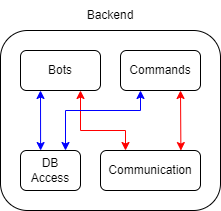
\includegraphics[width=0.35\textwidth]{img/backend_internals.png}
	\caption{Estructura interna del \textit{backend}.}
\end{figure}

\textbf{\textit{Worker}} Ejecuta los bots. Un \textit{worker} puede ejecutar N bots, y puede haber M \textit{workers} distintos. Compuesto por un componente para la ejecución de bots y por otro de comunicación. Los \textit{workers} se comunican directamente con el backend.

\begin{figure}[H]
	\centering
	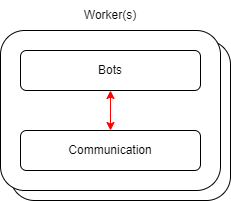
\includegraphics[width=0.35\textwidth]{img/worker_internals.png}
	\caption{Estructura interna de los \textit{workers}.}
\end{figure}


\textbf{\textit{Frontend}} Interfaz de usuario. Se comunica con el \textit{backend} mediante la \textit{API REST}. Compuesto por un componente para la gestión de bots, otro para la gestión de comandos y por otro de comunicación.

\begin{figure}[H]
	\centering
	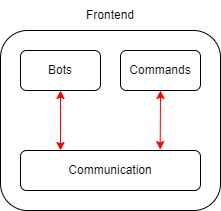
\includegraphics[width=0.35\textwidth]{img/frontend_internals.png}
	\caption{Estructura interna del \textit{frontend}.}
\end{figure}

Volviendo a las ventajas de la arquitectura, destaca en primer lugar la modularidad, ya que el \textit{backend} sería completamente independiente de la interfaz de usuario y de los \textit{workers}. Esto permitiría por un lado el desarrollo de distintas interfaces de usuario y por otro la posibilidad de escalar horizontalmente los \textit{workers} sin tener que escalar del mismo modo el \textit{backend}.


\subsection{Autenticación y seguridad}

Se ha decidido no incluir ningún sistema de autenticación en ninguno de los microservicios que lo conforma. Por lo tanto, podría decirse que el software es inseguro.

Implementar un sistema de autenticación implica la adición de una lógica extra que consume una serie de recursos, y puede ser algo que no sea necesario según dónde se implemente el sistema (e.g. una instalación local de pruebas o en el caso de este software, en la máquina local de un usuario). No implementando esta autenticación, se evita una implementación específica, que seguramente no case con los modelos usuales de autenticación.

Por otro lado, existen multitud de software y servicios que se dedican exclusivamente a la autenticación, y cuya integración con \textbf{Matroos} sería sencilla e incluiría esa capa de seguridad que falta. Algunos ejemplos son los siguientes:

\begin{itemize}
	\item \href{https://auth0.com/es}{\textit{Auth0}}
	\item \textit{LDAP} y/o (con \href{https://doc.traefik.io/traefik/}{\textit{Traefik}}, \href{https://www.nginx.com/}{\textit{NGinx}} u otros)
	\item \href{https://oauth.net/2/}{\textit{OAuth 2.0}}
	\item \href{https://firebase.google.com/?hl=es}{\textit{Firebase}}
	\item \href{https://aws.amazon.com/es/cognito/}{\textit{Amazon Cognito}}
\end{itemize}

\subsection{Posibles configuraciones del software}

En esta sección se presentan algunas posibles configuraciones del software, usando sus diferentes partes combinadas con servicios de autenticación.

\subsubsection{\textit{Backend} + \textit{frontend}}

Sistema completo sin autenticación. El usuario accede a la configuración del sistema mediante el \textit{frontend} y hace uso de los bots mediante los comandos en servidores de \textit{Discord}.

\begin{figure}[H]
	\centering
	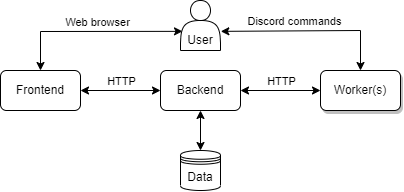
\includegraphics[width=0.8\textwidth]{img/architecture_with_frontend.png}
	\caption{Ejemplo de arquitectura compuesta por el \textit{backend} y el \textit{frontend}.}
\end{figure}

\subsubsection{\textit{Backend}}

Sistema sin autenticación ni \textit{frontend}. El usuario accede a la configuración del sistema mediante la \textit{API REST} que provee el \textit{backend} y hace uso de los bots mediante los comandos en servidores de \textit{Discord}.

\begin{figure}[H]
	\centering
	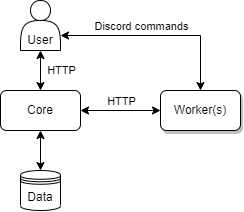
\includegraphics[width=0.4\textwidth]{img/architecture_without_frontend.png}
	\caption{Ejemplo de arquitectura compuesta sólo por el \textit{backend}.}
\end{figure}

\subsubsection{Autenticación externa + \textit{backend} + \textit{frontend}}

Sistema completo que cuenta con un \textit{middleware} para la autenticación de usuarios. Todas las peticiones que realiza el usuario pasan por este \textit{middleware}, que es el que autoriza o deniega que las peticiones lleguen al \textit{frontend} y por tanto al \textit{backend}.

\begin{figure}[H]
	\centering
	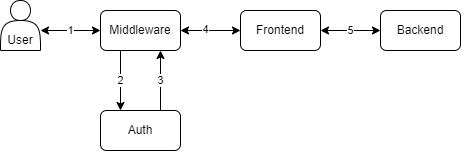
\includegraphics[width=0.8\textwidth]{img/auth_with_frontend.png}
	\caption{Ejemplo de arquitectura usando autenticación externa, el \textit{backend} y el \textit{frontend}.}
\end{figure}


\subsubsection{Autenticación externa + \textit{backend}}

Mismo caso que el anterior, pero sin intervención del \textit{frontend}.

\begin{figure}[H]
	\centering
	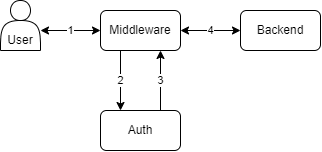
\includegraphics[width=0.6\textwidth]{img/auth_without_frontend.png}
	\caption{Ejemplo de arquitectura usando autenticación externa y el \textit{backend}.}
\end{figure}





\section{Bots}

Los bots son las entidades que pueden tener configurados una serie de comandos ejecutables a voluntad de los usuarios para automatizar tareas en un servidor de \textit{Discord}. Estos bots pueden agregarse a distintos servidores, pudiendo ser útiles en diversos contextos.

Los datos necesarios para definir un bot son los siguientes:

\begin{itemize}
	\item \verb|ID: Guid|. Identificador único del bot.
	\item \verb|Name: string|. Nombre del bot.
	\item \verb|Description: string|. Descripción del bot.
	\item \verb|Key: string|. \textit{Key} del bot. Clave necesaria para poder acceder a la \textit{API} de \textit{Discord}.
	\item \verb|Commands: List<Guid>|. Lista de comandos asociados al bot.
\end{itemize}





\section{Comandos}

Los comandos son las órdenes que se pueden configurar en un bot para que se ejecuten en ellos cuando el usuario quiere.

Como se indicaba en capítulos anteriores la intención es permitir la creación de comandos sencilla, y además la extensión del repertorio de comandos reutilizables disponibles. Para esto se han definido distintas entidades que permiten completar este cometido.

\subsection{\textit{UserCommand}}

Estos comandos son los que crean los usuarios para después asignarlos a los bots. Estos comandos pueden ser los tipos definidos en la sección \hyperref[sec:commandtype]{\textit{CommandType}}.

Sus parámetros necesarios son:

\begin{itemize}
	\item \verb|ID: Guid|. Identificador único del comando.
	\item \verb|Name: string|. Nombre del comando.
	\item \verb|Description: string|. Descripción del comando.
	\item \verb|Type: CommandType|. Tipo de comando.
	\item \verb|Trigger: string|. Activador del comando. Cadena que se escribe tras el prefijo para invocar este comando.
	\item \verb|Mode: CommandMode|. Modo de ejecución del comando.
	\item \verb|Parameters: Dictionary<string, object>|. Parámetros del comando.
\end{itemize}

\subsection{\textit{CommandMode}}

Modos de ejecución de comandos. Definen el modo en el que el comando se ejecuta y cuando deben aportarse los parámetros necesarios. Es importante destacar que no todos los comandos se pueden (o deben) ejecutar de todos los modos distintos.

\begin{itemize}
	\item \verb|INLINE|. Los parámetros del comando se introducen al ejecutar el comando.
	\item \verb|SCOPED|. Los parámetros del comando se introducen al crear el comando. El comando se ejecutará haciendo uso del \textit{trigger} del comando.
	\item \verb|HEADLESS|. Los parámetros del comando se introducen al crear el comando. El comando no se puede ejecutar manualmente.
	\item \verb|SINGLE|. El comando no necesita parámetros.
\end{itemize}

\subsection{\textit{CommandType}}
\label{sec:commandtype}

Esta lista es extensible y contiene los tipos de comandos reutilizables que van a estar disponibles para los usuarios en el sistema. En la primera versión funcional del software se proponen los siguientes tipos de comandos que podrían ser usados por todos los usuarios. Más detalles en las siguientes secciones.

\begin{itemize}
	\item \verb|MESSAGE|
	\item \verb|PING|
	\item \verb|STATUS|
	\item \verb|VERSION|
	\item \verb|TIMER|
\end{itemize}

\subsection{\textit{BaseCommand}}

Define las características básicas de un tipo de comando reutilizable. Estas son:

\begin{itemize}
	\item \verb|AllowedModes: List<CommandMode>|. Los modos de ejecución del comando permitidos.
	\item \verb|CommandType: CommandType|. El tipo de comando.
	\item \verb|NeedsPrefix: boolean|. Si el comando necesita ser invocado haciendo uso de un prefijo o no.
	\item \verb|Parameters: List<ParameterSignature>|. Los tipos de parámetros que necesita el comando.
\end{itemize}


\subsubsection{\textit{ParameterSignature}}

Define los parámetros que necesita un comando.

\begin{itemize}
	\item \verb|Name: string| Nombre del parámetro.
	\item \verb|DisplayName: string| Nombre (de visualización) del parámetro.
	\item \verb|Required: boolean| Si el parámetro es requerido o no.
	\item \verb|Type: DataType| El tipo de dato del parámetro.
	\item \verb|Default: Object| El valor por defecto.
	\item \verb|Validator: Func<object, bool>| Función para validar el parámetro.
\end{itemize}


\subsubsection{\textit{DataType}}

Tipos de datos asignables a los parámetros. Ayuda a los usuarios a comprender el tipo de dato que deben asignar a los comandos cuando éstos son creados. Esta lista podría extenderse si fuese preciso.

\begin{itemize}
	\item \verb|BOOLEAN|
	\item \verb|DATE|
	\item \verb|DOUBLE|
	\item \verb|INTEGER|
	\item \verb|STRING|
	\item \verb|LIST|
\end{itemize}


\subsection{\textit{Custom Commands}}

En esta sección se detallan en profundidad los cinco comandos que se proponen.

\subsubsection{\textit{MessageCommand}}

Envía un mensaje en un canal.

Parámetros:

\begin{table}[H]
    \centering
    \def\arraystretch{1.25}
    \begin{adjustbox}{max width=\textwidth}
    \begin{tabularx}{\textwidth}{|l|l|l|l|L|}
    \hline
        \textbf{\textit{Name}} & \textbf{\textit{DisplayName}} & \textbf{\textit{Type}} & \textbf{\textit{Default}} & \textbf{Definición} \\ \hline
    \hline
        Message & Message & string & ~ & Mensaje a enviar. \\ \hline
        ChannelID & ChannelID? & string & "" & Canal donde enviar el mensaje. Opcional, si no se indica se manda en el canal actual. \\ \hline
        IsResponse & IsResponse? & boolean & false & Si el mensaje se debe enviar como una respuesta al comando. \\ \hline
        IsTTS & IsTTS? & boolean & false & Si el mensaje se debe enviar como \textit{TTS} (\textit{Text to speach}) \\ \hline
    \end{tabularx}
    \end{adjustbox}
    \caption{Comando \textit{Message}.}
\end{table}

Configuración del comando:

\begin{itemize}
	\item \verb|AllowedModes|: \verb|CommandMode.SCOPED|
	\item \verb|NeedsPrefix|: \verb|true|
\end{itemize}


\subsubsection{\textit{PingCommand}}

Hace una petición \textit{ping} a un host.

Parámetros:

\begin{table}[H]
    \centering
    \def\arraystretch{1.25}
    \begin{adjustbox}{max width=\textwidth}
    \begin{tabularx}{\textwidth}{|l|l|l|l|L|}
    \hline
        \textbf{\textit{Name}} & \textbf{\textit{DisplayName}} & \textbf{\textit{Type}} & \textbf{\textit{Default}} & \textbf{Definición} \\ \hline
    \hline
        Host & Host & string & ~ & Host al que hacer el ping. \\ \hline
        ChannelID & ChannelID? & string & "" & Canal donde enviar el mensaje. Opcional, si no se indica se manda en el canal actual. \\ \hline
    \end{tabularx}
    \end{adjustbox}
    \caption{Comando \textit{Ping}.}
\end{table}

Configuración del comando:

\begin{itemize}
	\item \verb|AllowedModes|: \verb|CommandMode.INLINE| y \verb|CommandMode.SCOPED|
	\item \verb|NeedsPrefix|: \verb|true|
\end{itemize}


\subsubsection{\textit{StatusCommand}}

Devuelve el estado del bot.

Parámetros:

\begin{table}[H]
    \centering
    \def\arraystretch{1.25}
    \begin{adjustbox}{max width=\textwidth}
    \begin{tabularx}{\textwidth}{|l|l|l|l|L|}
    \hline
        \textbf{\textit{Name}} & \textbf{\textit{DisplayName}} & \textbf{\textit{Type}} & \textbf{\textit{Default}} & \textbf{Definición} \\ \hline
    \hline
        ChannelID & ChannelID? & string & "" & Canal donde enviar el mensaje. Opcional, si no se indica se manda en el canal actual. \\ \hline
    \end{tabularx}
    \end{adjustbox}
    \caption{Comando \textit{Status}.}
\end{table}

Configuración del comando:

\begin{itemize}
	\item \verb|AllowedModes|: \verb|CommandMode.SCOPED|
	\item \verb|NeedsPrefix|: \verb|true|
\end{itemize}


\subsubsection{\textit{VersionCommand}}

Devuelve la versión actual del bot.

No necesita parámetros.

Configuración del comando:

\begin{itemize}
	\item \verb|AllowedModes|: \verb|CommandMode.SINGLE|
	\item \verb|NeedsPrefix|: \verb|true|
\end{itemize}

\subsubsection{\textit{TimerCommand}}
Ejecuta un comando cada vez que se cumple el intervalo de tiempo.

Parámetros:

\begin{table}[H]
    \centering
    \def\arraystretch{1.25}
    \begin{adjustbox}{max width=\textwidth}
    \begin{tabularx}{\textwidth}{|l|l|l|l|L|}
    \hline
        \textbf{\textit{Name}} & \textbf{\textit{DisplayName}} & \textbf{\textit{Type}} & \textbf{\textit{Default}} & \textbf{Definición} \\ \hline
    \hline
        Interval & Interval & string (Cron) & ~ & Cron que indique cuando se debe ejecutar el comando. \\ \hline
        CommandID & CommandID & GUID & ~ & Comando a ejecutar. Debe ser de tipo SCOPED. \\ \hline
        Active & Active & boolean & ~ & Si el *timer* está activo o no. \\ \hline
    \end{tabularx}
    \end{adjustbox}
    \caption{Comando \textit{Timer}.}
\end{table}

Configuración del comando:

\begin{itemize}
	\item \verb|AllowedModes|: \verb|CommandMode.HEADLESS|
	\item \verb|NeedsPrefix|: \verb|false|
\end{itemize}


\subsection{Ejemplos de \textit{UserCommands}}

En las siguientes secciones se incluyen posibles configuraciones de cada uno de los comandos propuestos. Se utiliza notación \textbf{JSON} pues es sencilla de interpretar.

\subsubsection{\textit{PingCommand}}

\begin{lstlisting}[language=sh]
{
    "Id": "3F2504E0-4F89-11D3-9A0C-0305E82C3301",
    "Name": "Ping",
    "Description": "Pings a site and returns the response.",
    "Type": CommandType.PING,
    "Trigger": "ping",
    "Mode": CommandMode.INLINE,
    "Parameters": {},
    "CreatedAt": "01/01/2020",
    "UpdatedAt": "01/01/2020"
}
\end{lstlisting}

Entrada del usuario: !ping my-service.com

Respuesta del bot: The ping is 17ms.

\begin{lstlisting}[language=sh]
{
    "Id": "3F2504E0-4F89-11D3-9A0C-0305E82C3301",
    "Name": "Ping Document",
    "Description": "Pings my-site.com and returns the response.",    
    "Type": CommandType.PING,
    "Trigger": "ping",
    "Mode": CommandMode.SCOPED,
    "Parameters": {
        "Host": "my-site.com"
    },
    "CreatedAt": "01/01/2020",
    "UpdatedAt": "01/01/2020"
}
\end{lstlisting}

Entrada del usuario: !ping

Respuesta del bot: The ping is 13ms.



\subsubsection{\textit{MessageCommand}}

\begin{lstlisting}[language=sh]
{
    "Id": "message-command-id",
    "Name": "Send message",
    "Description": "Sends a message.",
    "Type": CommandType.MESSAGE,
    "Trigger": "message",
    "Mode": CommandMode.SCOPED,
    "Parameters": {
        "Message": "Hola!",
        "IsResponse": false,
        "ChannelID": null,
        "IsTTS": true
    },
    "CreatedAt": "01/01/2020",
    "UpdatedAt": "01/01/2020"
}
\end{lstlisting}

Entrada del usuario: !message

Respuesta del bot: (TTS) Hola!



\subsubsection{\textit{StatusCommand}}

\begin{lstlisting}[language=sh]
{
    "Id": "3F2504E0-4F89-11D3-9A0C-0305E82C3301",
    "Name": "Status",
    "Description": "Sends the bot status.",
    "Type": CommandType.STATUS,
    "Trigger": "status",
    "Mode": CommandMode.SCOPED,
    "Parameters": {
        "ChannelID": null
    },
    "CreatedAt": "01/01/2020",
    "UpdatedAt": "01/01/2020"
}
\end{lstlisting}

Entrada del usuario: !status

Respuesta del bot: Test Bot - Uptime: 10h


\pagebreak

\subsubsection{\textit{TimerCommand}}

\begin{lstlisting}[language=sh]
{
    "Id": "3F2504E0-4F89-11D3-9A0C-0305E82C3301",
    "Name": "Timer Greetings",
    "Description": "Sends the Greeting message every 10 minutes.",
    "Type": CommandType.TIMER,
    "Trigger": null,
    "Mode": CommandMode.HEADLESS,
    "Parameters": {
        "Interval": "* */10 * * * ?",
        "CommandID": "message-command-id",
        "Active": true
    },
    "CreatedAt": "01/01/2020",
    "UpdatedAt": "01/01/2020"
}
\end{lstlisting}

Entrada del usuario: (ninguna)

Respuesta del bot: (cada 10 segundos) Hola!



\subsubsection{\textit{VersionCommand}}

\begin{lstlisting}[language=sh]
{
    "Id": "3F2504E0-4F89-11D3-9A0C-0305E82C3301",
    "Name": "Version",
    "Description": "Sends the bot version",
    "Type": CommandType.VERSION,
    "Trigger": "version",
    "Mode": CommandMode.SINGLE,
    "Parameters": {},
    "CreatedAt": "01/01/2020",
    "UpdatedAt": "01/01/2020"
}
\end{lstlisting}

Entrada del usuario: !version

Respuesta del bot: Version 3.1.5





\subsection{\textit{User journeys}}

Volviendo a los \textit{user journeys} definidos en el capítulo 3, algunos de estos se pueden ampliar, incluyendo más información una vez han sido definidas características extra de los comandos.

\subsubsection{Crear un comando}

\begin{enumerate}
	\item El usuario solicita al sistema los comandos disponibles para crear.
	\item El sistema devuelve al usuario una lista que contiene los distintos comandos, además de los parámetros que necesitan cada uno de ellos.
	\item El usuario decide qué comando quiere crear, y provee al sistema de los datos necesarios.
	\item[!] Si ocurre algún error, el sistema cancela la creación del comando.
	\item El sistema crea el comando.
\end{enumerate}

\subsection{Ampliación del repertorio de comandos}

Para la realización de este \textit{user journey} es necesario el uso de C\#.

\begin{enumerate}
	\item El usuario define el nuevo tipo de comando (\textit{CommandType}).
	\item El usuario crea una nueva clase para ese comando. Ésta clase debe heredar de \textit{BaseCommand}, para obtener la funcionalidad básica.
	\item El usuario define los parámetros que necesita ese comando apoyándose en el tipo \textit{ParameterSignature} y \textit{DataType}.
	\item El usuario implementa la funcionalidad asociada al comando, esto es el código que se ejecuta cuando el comando es invocado.
	\item El comando queda disponible para ser usado por el sistema.
	\item[!] Es necesario reiniciar el sistema para que pueda utilizarse el nuevo comando.
\end{enumerate}


\section{Base de datos}

En esta sección se definen las diferentes colecciones de datos que se utilizan para almacenar los datos necesarios en \textbf{Matroos}.

\subsection{Bots}

Almacena los datos asociados a los bots creados por los usuarios.

\begin{figure}[H]
	\centering
	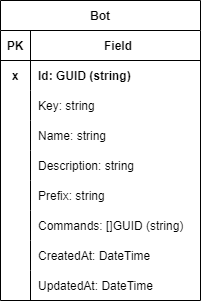
\includegraphics[width=0.3\textwidth]{img/database_architecture_bot.png}
	\caption{Colección de datos que almacena los bots.}
\end{figure}

\subsection{Comandos}

Almacena los datos asociados a los comandos creados por los usuarios.

\begin{figure}[H]
	\centering
	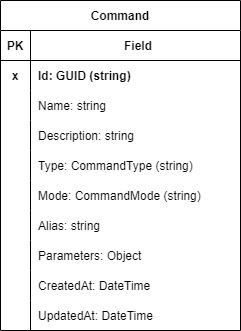
\includegraphics[width=0.3\textwidth]{img/database_architecture_command.png}
	\caption{Colección de datos que almacena los camandos.}
\end{figure}

